% !TeX encoding = UTF-8
% !TeX program = pdflatex
% !TeX spellcheck = en_EN
\documentclass[Lau,oneside,noexaminfo]{sapthesis} % LaM for a Laurea Magistrale
\usepackage{microtype}
\usepackage[utf8]{inputenc}
\usepackage[hidelinks]{hyperref}
\usepackage{graphicx}
\usepackage{tabularx}
\usepackage{ltablex}
\usepackage{longtable}
\usepackage{booktabs}
\usepackage{siunitx}
\usepackage{ltxtable}
\usepackage{float}
\usepackage{algorithm}
\usepackage{algorithmic}
\usepackage{listings}
\usepackage{setspace}
\usepackage{caption}
\usepackage{subcaption}

\graphicspath{ {./images/} }

\setlength{\parindent}{0em}
\setlength{\parskip}{0.36em}

\hypersetup{pdftitle={Deep Deterministic Policy Gradient for Regularity Rally in TORCS Simulator},pdfauthor={Alessio Ragno}}
\title{Deep Deterministic Policy Gradient for Regularity Rally in TORCS Simulator}
\author{Alessio Ragno}
\IDnumber{1759198}
\course{Ingegneria Informatica e Automatica}
\courseorganizer{Facoltà di Ingegneria dell'Informazione, Informatica e Statistica\\Dipartimento di Ingegneria Informatica, Automatica e Gestionale}
\AcademicYear{2018/2019}
\copyyear{2019}
\advisor{Prof. Roberto Capobianco}
\authoremail{ragno.1759198@studenti.uniroma1.it, spideralessio97@gmail.com}

\definecolor{mygreen}{rgb}{0,0.6,0}
\definecolor{mygray}{rgb}{0.5,0.5,0.5}
\definecolor{mymauve}{rgb}{0.58,0,0.82}
\definecolor{lightgray}{rgb}{0.95,0.95,0.95}

\lstset{ %
  backgroundcolor=\color{lightgray},   % choose the background color
  basicstyle=\footnotesize,        % size of fonts used for the code
  breaklines=true,                 % automatic line breaking only at whitespace
  captionpos=b,                    % sets the caption-position to bottom
  commentstyle=\color{mygreen},    % comment style
  escapeinside={\%*}{*)},          % if you want to add LaTeX within your code
  keywordstyle=\color{blue},       % keyword style
  stringstyle=\color{mymauve},     % string literal style
  language=python,
  numbers=left
}

\begin{document}

\frontmatter
\maketitle
\dedication{Dedicated to\\the ones that supported me in my experience}
\begin{abstract}
This thesis is the result for the Excellence Course Project which was developed during the last year of the degree.

The aim of this thesis is to study an application of Deep Reinforcement Learning by training a sensor-based autonomous car to drive in a Regularity Rally, which is, a type of motor sport race with the purpose of driving in the minimum time at a specified average speed. In order to achieve the goal, Deep Deterministic Policy Gradient (DDPG) algorithm has been applied.

This report will briefly introduce Reinforcement Learning theory, show how the project has been implemented and its results.

A parallel project focusing on Speed Racing has been developed by Dylan Savoia.

\end{abstract}
\begin{spacing}{0}
\tableofcontents
\end{spacing}
\mainmatter
\chapter{Introduction}
Reinforcement Learning is a branch of Artificial Intelligence that studies algorithms to teach an agent how to act in an environment. Some applications of this subject are robotics, advertising, business and chemistry. For instance, Mariya et al. used Deep Reinforcement learning to generate new molecules for drug design. \cite{TROPSHA}

In most cases reinforcement learning algorithms are initially applied on games which, generally, represent complex environments which can easily become suitable for Reinforcement Learning problems. Important examples of games impact on Reinforcement Learning are chess and GO: beating humans on these two strategy games, in facts, have been the first challenges of Reinforcement Learning. 

For this project the environment chosen is TORCS, an open source car simulator that can be easily controlled through Python APIs.

\chapter{TORCS}
TORCS (The Open Racing Car Simulator) is an open-source 3D car racing simulator released in 1997 and developed by Bernhard Wymann (project leader), Christos Dimitrakakis (simulation, sound, AI) and Andrew Sumner (graphics, tracks).
\begin{figure}[H]
\caption{Classic View of a TORCS car in a race}
\centering
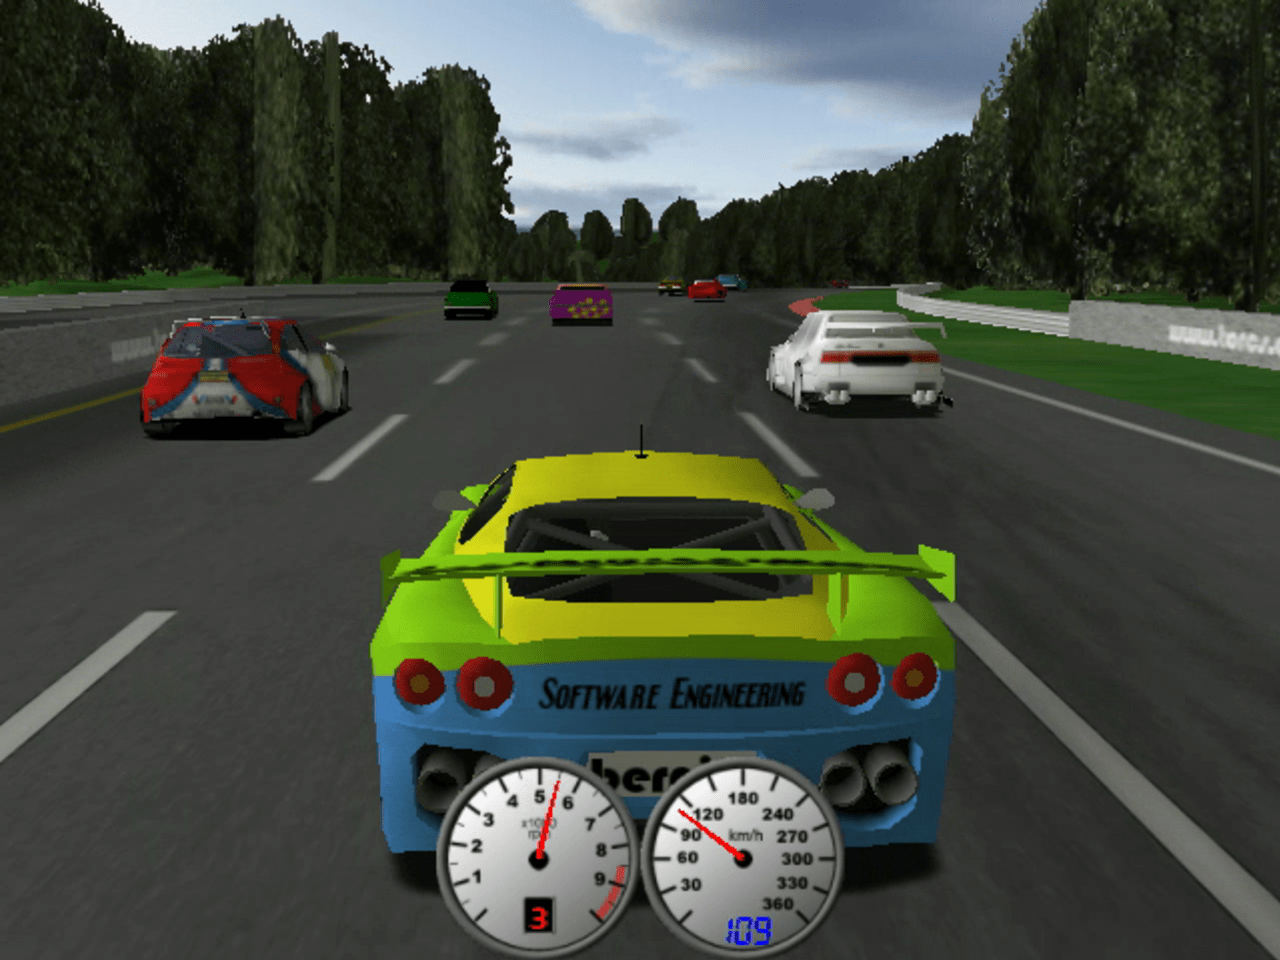
\includegraphics[width=0.7\textwidth]{torcs}
\end{figure}
\section{Simulated Car Racing Championship}
\label{SCR}
Simulated Car Racing Championship (SCRC) is an international competition with the purpose to design a pre-programmed driver which can compete on unknown tracks either alone or against other virtual drivers.

The drivers perceive the environment through a number of sensors that describe relevant features describing the car surroundings (e.g., the track limits, the position of near-by obstacles), the car state (the fuel level, the engine RPMs, the current gear, etc.), and the current game state (lap time, number of lap, etc.).

The competition software extends the original TORCS architecture by adding a client-server module, real time events simulation and an abstraction layer between the driver code and the race server. \cite{SCR}

\begin{longtable}{p{0.15\textwidth}p{0.25\textwidth}p{0.5\textwidth}}
\caption{Description of TORCS available sensors}\\
\toprule
\textbf{Name}          & \textbf{Range}            & \textbf{Description}    \\
\midrule
\endfirsthead
\caption{Description of TORCS available sensors (continued)}\\
\toprule
\textbf{Name}          & \textbf{Range}            & \textbf{Description}    \\
\midrule
\endhead
\bottomrule
\endfoot
angle         & $[-\pi, +\pi]$ (rad)  & Angle between the car direction and the direction of the track axis      \\
curLapTime    & $[0, +\infty)$ (s)      & Time elapsed during current lap    \\
damage        & $[0, +\infty)$ (point)  & Current damage of the car    \\
distFromStart & $[0, +\infty)$ (m)      & Distance of the car from the start line along the track line             \\
distRaced     & $[0, +\infty)$ (m)       & Distance covered by the car from the beginning of the race \\
focus         & $[0, 200]$ (m)      & Vector of 5 range finder sensors: each sensor returns the distance between the track edge and the car within a range of 200 meters   \\
fuel          & $[0, +\infty)$ (l)       & Current fuel level           \\
gear          & ${-1, 0, 1, \dots\, 6}$ & Current gear: -1 is reverse, 0 is neutral and the gear from 1 to 6       \\
lastLapTime   & $[0, +\infty)$ (s)       & Time to complete the last lap\\
opponents     & $[0, 200]$ (m)      & Vector of 36 opponent sensors.     \\
racePos       & ${1, 2, \dots\, N}$    & Position in the race with respect to other cars  \\
rpm           & $[0, +\infty)$ (rpm)     & Number of rotation per minute of the car engine  \\
speedX        & $(-\infty, +\infty)$ (km/h)   & Speed of the car along the longitudinal axis of the car.   \\
speedY        & $(-\infty, +\infty)$ (km/h)   & Speed of the car along the transverse axis of the car\\
speedZ        & $(-\infty, +\infty)$ (km/h)   & Speed of the car along the Z axis of the car     \\
track         & $[0, 200]$ (m)      & Vector of 19 range finder sensors: each sensors returns the distance between the track edge and the car within a range of 200 meters \\
trackPos      & $(-\infty, +\infty)$          & Distance between the car and the track axis      \\
wheelSpinVel  & $[0, +\infty)$ (rad/s)  & Vector of 4 sensors representing the rotation speed of wheels \\
z             & $(-\infty, +\infty)$ (m)      & Distance of the car mass center from the surface of the track along the Z axis \\
\end{longtable}
\begin{longtable}{p{0.15\textwidth}p{0.25\textwidth}p{0.5\textwidth}}
\caption{Description of TORCS available effectors}\\
\toprule
\textbf{Name}          & \textbf{Range}            & \textbf{Description}    \\
\midrule
\endfirsthead
\caption{Description of TORCS available effectors (continued)}\\
\toprule
\textbf{Name}          & \textbf{Range}            & \textbf{Description}    \\
\midrule
\endhead
\bottomrule
\endfoot
accel         & $[0, 1]$  & Virtual gas pedal       \\
brake         & $[0, 1]$  & Virtual brake pedal \\
clutch        & $[0, 1]$  & Virtual clutch pedal    \\
gear    & ${1, 2, \dots\, 6}$      & Gear Value \\
steering        & $[-1, 1]$  & Steering value    \\
focus    & $[-90, 90]$     & Focus direction \\
meta        & ${0, 1}$  & Ask competition to restart the race    \\
\end{longtable}

\chapter{Reinforcement Learning}
Machine Learning is an application of Artificial Intelligence which studies algorithms and methods that can automatically learn and improve through experience without being explicitly programmed. 

Typically, Machine Learning methods are divided in three main categories: supervised learning, unsupervised learning and reinforcement learning (RL). 

The former’s purpose is to learn a mapping from inputs $x$ to outputs $y$, given a labeled set of known input-output pairs called training set; the second focuses on finding “interesting patterns” in data; \cite{MURPHY} the latter, is the problem faced by an agent that must learn behavior through trial-and-error interactions with a dynamic environment. 

In the standard RL model, also known as Markov Decision Process (MDP), an agent is connected to an environment it can interact with. Every time an action is executed, the agent receives its current state in the environment with the gained reward, that can be positive or negative. 

Formally, in MDP a model is defined by:
\begin{itemize}
  \item a set of environment states $S$
  \item a set of agent actions $A$
  \item a set of scalar rewards $R$
\end{itemize}
RL focuses to learn a behavior that maximizes the expected cumulative reward. \cite{RLSURVEY} 

\begin{figure}[H]
\caption{The agent-environment interaction in a Markov decision process \cite{SUTTONBARTO}}
\centering
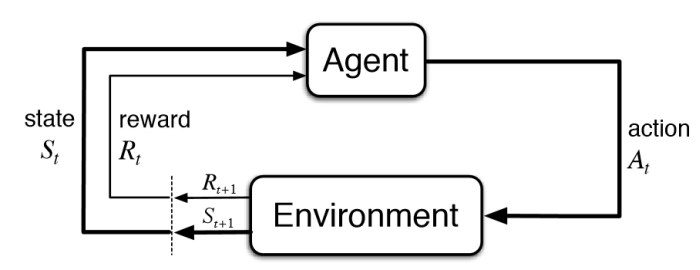
\includegraphics[width=\textwidth]{markov}
\end{figure}
The cumulative reward at each time step  t can be written as:
\begin{equation}
G_t = R_{t+1} + R_{t+2} + \dots\ = \sum_{k=0}^{T}R_{t+k+1}
\label{finitehorizon}
\end{equation}
Equation \ref{finitehorizon} is also called finite-horizon model, but it is not always appropriate: in many cases the precise length of the agent's life is unknown in advance, so it is preferable to use the infinite-horizon discounted model, as defined in equation \ref{infinitehorizon}:
\begin{equation}
G_t = \sum_{k=0}^{\infty}\gamma^k R_{t+k+1}
\label{infinitehorizon}
\end{equation}
The infinite-horizon discounted model takes into account the long-run reward of the agent, but the future received rewards are geometrically discounted according to discount factor $\gamma$.
The expected return given a certain state-action tuple is called value function (equation \ref{value}).
\begin{equation}
V(s,a) = E[G_t \mid S_t=s, A_t = a]
\label{value}
\end{equation}
\section{Bellman Equation}
The value learned at time $t$ strongly depends on the function learned at time $t-1$, this relation is described by the Bellman Equation:
\begin{align}
V(s, a) &= E[G_t \mid S_t=s, A_t = a] \\
&= E[R_{t+1} + \gamma R_{t+2} + \gamma^2 R_{t+3} + \dots \mid S_t=s, A_t = a] \\
&= E[R_{t+1} + \gamma (R_{t+2} + \gamma R_{t+3} + \dots) \mid S_t=s, A_t = a] \\
&= E[R_{t+1} + \gamma G_{t+1} \mid S_t=s, A_t = a] \\
&= E[R_{t+1} + \gamma V(S_{t+1}) \mid S_t=s, A_t = a]
\label{bellman}
\end{align}
\section{Monte Carlo and TD Learning}
A RL model can be learned in two ways:
\begin{itemize}
	\item Monte Carlo: rewards are given at the end of the game and the agent learns on the cumulative reward.
	\begin{equation}
V( S_t ) = V( S_t ) + \alpha[ G_t - V(S_t) ]
	\end{equation}
	\item Temporal Difference (TD) Learning: every step the agent gets the reward and model is updated.
	\begin{equation}
V( S_t ) = V( S_t ) + \alpha[ R_{t+1} + \gamma V(S_t+1)- V(S_t) ]
	\end{equation}
\end{itemize}
With long episodes TD Learning is preferable as using only the cumulative reward might penalize good actions chosen in bad episodes and reward bad actions taken in good episodes.


\section{Approaches to solve a RL problem}
There are three main approaches to solve a RL problem: value based, policy based and model based. 

Following these three methods take place others are generated, such as actor critic.
\subsection{Value based}
Value based class of algorithms aims to build a value function of states (or of state-action pairs) that estimate “how good” it is for the agent to be in a given state (or how good it is to perform a given action in a given state). The notion of “how good” here is defined in terms of expected future rewards. One of the simplest and most popular value based algorithms is Q-learning (Watkins, 1989). 

Q-learning keeps a lookup table of values $Q(s,a)$ with one entry for every state-action pair that estimates the  expected cumulative reward. The value function Q can be defined in equation \ref{qfunction}.
\begin{equation}
Q( s,a ) = E( \sum_{k=0}^{\infty} \gamma^k r_t+k \mid s_t=s, a_t=a )
\label{qfunction}
\end{equation}
Once the value function is known (or estimated) it is possible to apply $argmax$ to select the most suitable action which would give the highest reward in a specific state.
\subsection{Policy based}
In policy based Reinforcement Learning the goal is to optimize the policy function $\pi$ without using a value function. The policy takes in input the state and returns the action the agent should take:
\begin{equation}
a = \pi(s)
\end{equation}
It is possible to define a deterministic policy, which returns the same action at a given state or a stochastic one  that outputs a distribution probability over actions at a given state.
\subsection{Model based}
Model based algorithms goal is to build a model of the environment in order to take the right action at a given state. This approach is less general than the other two, in facts, for every environment it is necessary to build a specific model.
\subsection{Actor-Critic}
If the value function is learned in addition to the policy, the Actor-Critic algorithm results:
\begin{itemize}
	\item Critic: updates value function parameters w and depending on the algorithm it could be action-value $Q(a\mid s,w)$ or state-value $V(s,w)$.
	\item Actor: updates policy parameters $\theta$, in the direction suggested by the critic, $\pi(a\mid s,\theta)$.
\end{itemize}
This class of algorithms is very powerful and it is the one this study will focus th is implemented in Deep Deterministic Policy Gradient (DDPG).
\chapter{Reinforcement Learning Algorithms Improvements}
This section focuses on some improvements that could be adopted while implementing a RL algorithm in order to improve performance and handle problems that could be encountered.
\section{Deep Learning}
The application of Neural Networks (NN) in RL gave place to Deep Reinforcement Learning. NNs to model policies and value functions is easier to handle continuous domain states and actions. An important example of this approach is Deep Q-Learning.
\subsection{Deep Q-Learning}
Deep Q-Learning is an improvement of Q-Learning in which NN is used to estimate the value function. Q-Learning can only be used with discrete actions and states while its deep version allows also continuous inputs.
\section{Target Function}
When using TD value based models, and in particular Deep Q-Learning, the value learned at time $t$ has a strong dependency on the function learned at time $t-1$ as pointed out by the Bellman Equation (equation \ref{bellman}).  

For Q-Learning, the Bellman Equation is expressed in equation \ref{bellmanqlearning}:
\begin{equation}
NewQ( s,a ) = Q( s,a ) + \alpha [ R(s,a) + \gamma maxQ(s',a') - Q(s,a) ]
\label{bellmanqlearning}
\end{equation}
The new Q value for a state-action tuple is the current Q value plus the learning rate $\alpha$ times the reward for taking that action at that state added to the difference between the discounted  maximum expected future reward given the next state-action tuple and the current Q value. 

What value based models try to do is minimize the error between real value function and the estimated one. The error is calculated by taking the difference between predicted Q target (maximum possible value from the next state) and the current Q value. NN parameters are updated by multiplying the error and gradient of the Q value:
\begin{equation}
\Delta w = \alpha [ (R + \gamma max_a Q(s',a,w)) - Q(s,a,w)] \nabla_w Q( s,a,w )
\end{equation}
Considering Q target is not known, it needs to be estimated together with the Q value, but using the same same weights for estimating both makes a big correlation between the target and the error that leads to slow learning. 

Instead of using the same weights, Google DeepMind introduced the notion of fixed Q-targets, which is, the use of a separate network with a fixed parameter for estimating the target that is updated every $\tau$ step by copying the same parameters of the Q Network.
\section{Exploration-Exploitation trade off}
Since RL tries to maximize the cumulative reward, frequently the model reaches local maximum points, which is mostly caused by a greedy behavior of the model that try to exploits current knowledge that is initially weak.

To avoid the model to exploit the “closest” source of rewards, in the training phase, it is necessary to add some noise to the actions in order to allow the agent to explore the entire environment and reach a better maximum point.

This problem is well-known as the “dilemma of exploration and exploitation”. \cite{SUTTONBARTO} A classic approach to partially solve this problem is the $\epsilon$-greedy policy: every step with probability $\epsilon$ a greedy action is taken and with probability $1 - \epsilon$ a non-greedy random action is taken.  
\section{Replay Buffer}
Replay Buffer or Experience Replay is a technique consisting in keeping buffer that stores the tuples (s, a, r, s’) of the various steps. 

At each step, the training routine picks a batch of samples from the buffer and uses them to update the model. This is quite useful because avoids forgetting previous experiences and reduces correlation between experiences.


\chapter{Deep Deterministic Policy Gradient}
\label{DDPG}
\begin{algorithm}[H]
    \caption{Deep Deterministic Policy Gradient}
\begin{algorithmic}[0]
\STATE Randomly initialize critic network $Q(s,a\mid\theta^Q)$ and actor $\mu(s\mid\theta^\mu)$ with weights $\theta^Q$ and $\theta^\mu$
\STATE Initialize target network $Q'$ and $\mu'$ with weights $\theta^{Q'} \gets \theta^{Q}$, $\theta^{\mu'} \gets \theta^{\mu}$
\STATE Initialize replay buffer $R$
\FOR{episode = 1, M}
    \STATE Initialize a random process $N$ for action exploration
    \STATE Receive initial observation state $s_1$
    \FOR{t = 1, T}
        \STATE Select action $a_t=\mu(s_t \mid \theta^\mu) + N_t$ according to the current policy and exploration noise
       	\STATE Execute action $a_t$ and observe reward $r_t$ and new state $s_t$
        \STATE Store transition $(s_t, a_t, r_t, s_{t+1})$ in $R$
        \STATE Sample a mini-batch of $n$ transitions $(s_i, a_i, r_i, s_{i+1})$ from $R$
        \STATE Set $y_i = r_i + \gamma Q'(s_{i+1}, \mu'(s_{i+1} \mid \theta^{\mu'})\mid \theta^{Q'})$
        \STATE Update critic by minimizing the loss $L={1 \over n} \sum_i (y_i - Q(s_i, a_i \mid \theta^Q))^2$
        \STATE Update the actor policy using the sampled policy gradient $$ \nabla_{\theta \mu}J \approx {1 \over n} \sum_i \nabla_a Q(s,a \mid \theta^Q) \mid_{s=s_i, a=\mu(s_i)} \nabla_{\theta \mu} \mu(s \mid \theta^\mu) \mid_{s_i}$$
        \STATE Update the target networks: $$\theta^{Q'} \gets \tau \theta^{Q} + (1-\tau)\theta^{Q'}$$ $$\theta^{\mu'} \gets \tau \theta^{\mu} + (1-\tau)\theta^{\mu'}$$
    \ENDFOR
\ENDFOR
\end{algorithmic}
\end{algorithm}
In 2016 Google Deepmind Researches created an algorithm based on the actor critic approach to apply Reinforcement Learning in environments with continuous action domain and continuous action spaces: Deep Deterministic Policy Gradient (DDPG).

Described in the paper “Continuous control with Deep Reinforcement Learning”, DDPG is the mixture of Deep Q-Learning and Deterministic Policy Gradient.\cite{DDPG}

DDPG, like Q-Learning, uses a replay buffer $R$ to store samples and implements separate target networks to calculate $y_t$ that are soft updated every step by a factor $\tau$\
\chapter{Implementation}
Here is the Project Implementation with some pieces of code and instructions to allow the reader to replicate it.
\section{Environment}
As explained in Section \ref{SCR}, the environment is completely developed in the SCRC available at the following Git Hub repository including a readme file that explains its compilation and installation: \url{https://github.com/fmirus/torcs-1.3.7}.
To interact with the simulator the developer Naoto Yoshida created a Python API that allows programmers to communicate with the environment with OpenAI-like methods. A detailed readme of the API is available at the following link: \url{https://github.com/ugo-nama-kun/gym_torcs}.
Here is a small piece of code that shows how gym torcs can be used to drive a TORCS car.

\begin{lstlisting}
from gym_torcs import TorcsEnv

#### Generate a Torcs environment
env = TorcsEnv(vision=False, throttle=True)

# reset environment
ob = env.reset()

# choose an action [steering, throttle, brake]
action = [0., 1., 0.]

# single step
ob, reward, done, _ = env.step(action)

# shut down torcs
env.end()
\end{lstlisting}
\section{DDPG in Tensorflow}
DDPG implementation has been implemented in Python Tensorflow using the Keras high-level API. The code has not been written from scratch, but starting from an old implementation based on the old version of Keras that is now deprecated. The original project owned by Ben Lau can be found at the following link: \url{http://yanpanlau.github.io/2016/10/11/Torcs-Keras.html}
\subsection{Critic Network}
Critic Network (CN) consists in a class containing four methods.
The constructor \_\_init\_\_ that initializes the parameters and instatiates the Critic Network and the Target Critic Network.
\begin{lstlisting}
class CriticNetwork(object):
  def __init__(self, sess, state_size, action_size, BATCH_SIZE, TAU, LEARNING_RATE):
    self.sess = sess
    self.BATCH_SIZE = BATCH_SIZE
    self.TAU = TAU
    self.LEARNING_RATE = LEARNING_RATE
    self.action_size = action_size
    K.set_session(sess)
    self.model, self.action, self.state = self.create_critic_network(state_size, action_size)  
    self.target_model, self.target_action, self.target_state = self.create_critic_network(state_size, action_size)  
    self.action_grads = tf.gradients(self.model.output, self.action)  #GRADIENTS for policy update
    self.sess.run(tf.initialize_all_variables())
\end{lstlisting}
The gradients method evaluates estimated value gradient on actions to train the Actor Network.
\begin{lstlisting}[firstnumber=13]
  def gradients(self, states, actions):
    return self.sess.run(self.action_grads, feed_dict={
      self.state: states,
      self.action: actions
    })[0]
\end{lstlisting}
target\_train that updates target network as explained in Section \ref{DDPG}
\begin{lstlisting}[firstnumber=18]
  def target_train(self):
    critic_weights = self.model.get_weights()
    critic_target_weights = self.target_model.get_weights()
    for i in range(len(critic_weights)):
      critic_target_weights[i] = self.TAU * critic_weights[i] + (1 - self.TAU)* critic_target_weights[i]
    self.target_model.set_weights(critic_target_weights)
\end{lstlisting}
create\_critic\_network method builds the Critic Neural Network by concatenating the input layers (state and action) with two hidden layers made respectively of 300 and 600 neurons.
\begin{lstlisting}[firstnumber=24]
  def create_critic_network(self, state_size,action_dim):
    S = Input(shape=[state_size], name='State')  
    A = Input(shape=[action_dim], name='Action')   
    w1 = Dense(HIDDEN1_UNITS, activation='relu', name='DenseLayerS0')(S)
    a1 = Dense(HIDDEN2_UNITS, activation='linear', name='DenseLayerA')(A) 
    h1 = Dense(HIDDEN2_UNITS, activation='linear', name='DenseLayerS1')(w1)
    h2 = add([h1,a1], name='DenseLayerAS0')    
    h3 = Dense(HIDDEN2_UNITS, activation='relu', name='DenseLayerAS1')(h2)
    V = Dense(action_dim,activation='linear', name='Value')(h3)   
    model = Model(inputs=[S,A],outputs=V)
    adam = Adam(lr=self.LEARNING_RATE)
    model.compile(loss='mse', optimizer=adam)
    return model, A, S
\end{lstlisting}
\begin{figure}[H]
\caption{Tensorboard graph of Critic Network}
\centering
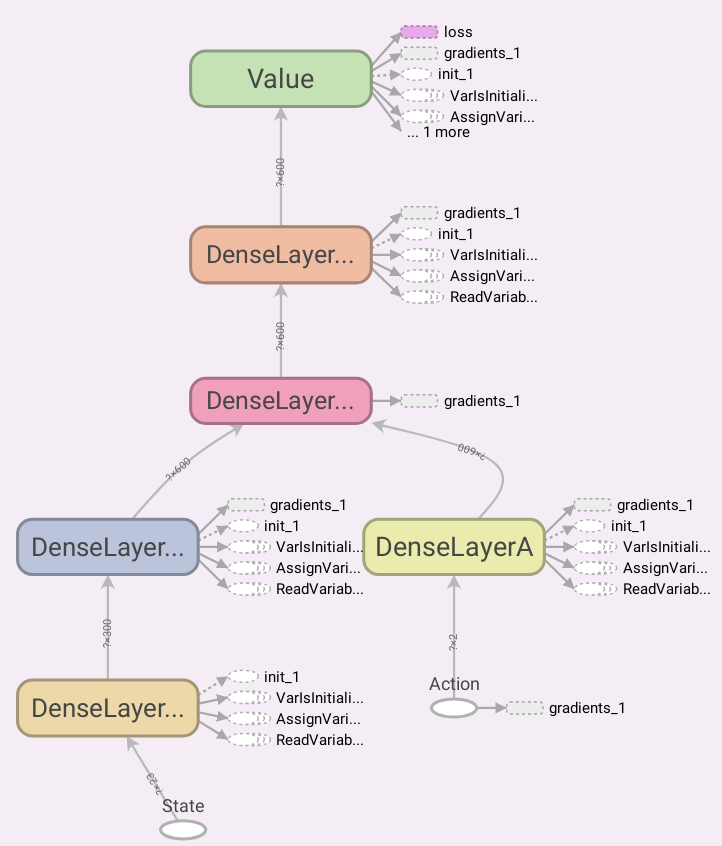
\includegraphics[width=0.8\textwidth]{critic}
\end{figure}
\section{Actor Network}
Actor Network (AN) realization is quite similar except for training method and the neural network initialization routine. In facts, the neural network input is just the agent state and the output is composed of the three commands the agent every step controls. The full implementation is provided in the next piece of code.
\begin{lstlisting}
class ActorNetwork(object):
  def __init__(self, sess, state_size, action_size, BATCH_SIZE, TAU, LEARNING_RATE):
    self.sess = sess
    self.BATCH_SIZE = BATCH_SIZE
    self.TAU = TAU
    self.LEARNING_RATE = LEARNING_RATE
    K.set_session(sess)
    self.model , self.weights, self.state = self.create_actor_network(state_size, action_size)   
    self.target_model, self.target_weights, self.target_state = self.create_actor_network(state_size, action_size) 
    self.action_gradient = tf.placeholder(tf.float32,[None, action_size])
    self.params_grad = tf.gradients(self.model.output, self.weights, -self.action_gradient)
    grads = zip(self.params_grad, self.weights)
    self.optimize = tf.train.AdamOptimizer(LEARNING_RATE).apply_gradients(grads)
    self.sess.run(tf.initialize_all_variables())

  def train(self, states, action_grads):
    self.sess.run(self.optimize, feed_dict={
      self.state: states,
      self.action_gradient: action_grads
    })

  def target_train(self):
    actor_weights = self.model.get_weights()
    actor_target_weights = self.target_model.get_weights()
    for i in range(len(actor_weights)):
      actor_target_weights[i] = self.TAU * actor_weights[i] + (1 - self.TAU)* actor_target_weights[i]
    self.target_model.set_weights(actor_target_weights)

  def create_actor_network(self, state_size,action_dim):
    S = Input(shape=[state_size])   
    h0 = Dense(HIDDEN1_UNITS, activation='relu')(S)
    h1 = Dense(HIDDEN2_UNITS, activation='relu')(h0)
    Steering = Dense(1,activation='tanh',kernel_initializer=variance_scaling(scale=1e-4, distribution='normal'), bias_initializer=variance_scaling(scale=1e-4, distribution='normal'))(h1)
    Acceleration = Dense(1,activation='tanh', kernel_initializer=variance_scaling(scale=1e-4, distribution='normal'), bias_initializer=variance_scaling(scale=1e-4, distribution='normal'))(h1)
    V = concatenate([Steering,Acceleration])         
    model = Model(inputs=S, outputs=V)
    return model, model.trainable_weights, S
\end{lstlisting}
\clearpage
Since acceleration and brake take values between 0 and 1 and steering value is between -1 and 1, in create\_actor\_network method, the Critic Network output layer parameters are initialized with a normal distribution scaled of a 1e-4 factor.
\begin{figure}[H]
\caption{Tensorboard graph of Actor Network}
\centering
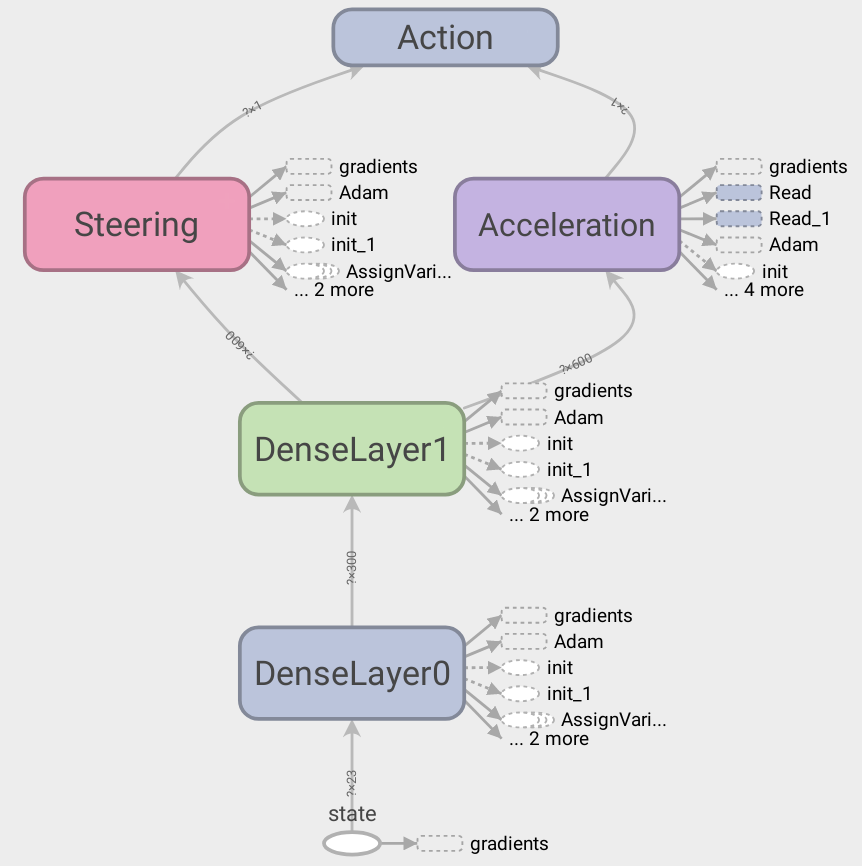
\includegraphics[width=0.8\textwidth]{actor}
\end{figure}
\section{Model Update}
The main work is done by the updated routine that is run right after an action is taken every step.
At first the environment is reset and the first state is stored observed.
\begin{lstlisting}
ob = env.reset()
s_t = np.hstack((ob.angle, ob.track, ob.trackPos, ob.speedX, env.wanted_speed))
\end{lstlisting}
After that, a loop over the max number of steps starts. The actor predicts an action, to which some noise is added and the agent interacts with the environment by sending the chosen action and a new observation is made.
\begin{lstlisting}[firstnumber=3]
for j in range(max_steps):
  epsilon -= 1.0 / EXPLORE
  a_t = np.zeros([1,action_dim])
  noise_t = np.zeros([1,action_dim])
  a_t_original = actor.model.predict(s_t.reshape(1, s_t.shape[0]))
  noise_t[0][0] = train_indicator * max(epsilon, 0) * OU.function(a_t_original[0][0],  0.0 , 0.60, 0.10)
  noise_t[0][1] = train_indicator * max(epsilon, 0) * OU.function(a_t_original[0][1],  0.7 , 1.00, 0.10)
  if random.random() <= 0.1 and train_indicator:
    print("********Now we apply the brake***********")
    noise_t[0][1] = train_indicator * max(epsilon, 0) * OU.function(a_t_original[0][1],  -0.1, 1.00, 0.10)
  for x in range(action_dim):
    a_t[0][x] = a_t_original[0][x] + noise_t[0][x]
  steering = a_t[0][0]
  acceleration = a_t[0][1] if a_t[0][1] >= 0 else 0.
  brake = abs(a_t[0][1]) if a_t[0][1] < 0 else 0.
  performed_action = [steering, acceleration, brake]
  ob, r_t, done, info = env.step(performed_action)
  s_t1 = np.hstack((ob.angle, ob.track, ob.trackPos, ob.speedX, env.wanted_speed))
\end{lstlisting}
The tuple (state, action, reward, next\_state) is then stored in the replay buffer. A batch of samples is picked from the replay buffer and for each sample the Target Q value is calculated, as well as the real value. 

Critic is trained by minimizing the mean squared error by the estimated Q value and the calculated Q value. Actor update is more complex: for every sample, actor predicts the action for the state and the value gradient is calculated on it, after that actor is trained by maximizing the value function over the state-action tuple. 

Finally, Target networks are updated.
\begin{lstlisting}[firstnumber=20]
  buff.add(s_t, a_t[0], r_t, s_t1, done)
  batch = buff.getBatch(BATCH_SIZE)
  states = np.asarray([e[0] for e in batch])
  actions = np.asarray([e[1] for e in batch])
  rewards = np.asarray([e[2] for e in batch])
  new_states = np.asarray([e[3] for e in batch])
  dones = np.asarray([e[4] for e in batch])
  y_t = np.asarray([e[1] for e in batch])
  target_q_values = critic.target_model.predict([new_states, actor.target_model.predict(new_states)]) 
  for k in range(len(batch)):
    if dones[k]:
      y_t[k] = rewards[k]
    else:
      y_t[k] = rewards[k] + GAMMA*target_q_values[k]
  if (train_indicator):
    loss += critic.model.train_on_batch([states,actions], y_t) 
    a_for_grad = actor.model.predict(states)
    grads = critic.gradients(states, a_for_grad)
    actor.train(states, grads)
    actor.target_train()
    critic.target_train()
  total_reward += r_t
  s_t = s_t1
\end{lstlisting}
\section{Ornstein–Uhlenbeck Noise}
To avoid the model to exploit and guarantee exploration Ornstein–Uhlenbeck (OU) Noise is used. The definition  and its implementation are the following:
\begin{equation}
\di x_t = \theta(\mu - x_t)\di t + \sigma \di W_t
\end{equation}
\begin{lstlisting}
class OU(object):
  def function(self, x, mu, theta, sigma):
    return theta * (mu - x) + sigma * np.random.randn(1)
\end{lstlisting}
$\theta$  means how “fast” the variable reverts towards the mean. $\mu$ represents the equilibrium or the mean value. $\sigma$ is the degree of volatility of the noise.
In the project the chosen parameters for steering, acceleration and brake are the following:
\begin{longtable}{p{0.225\textwidth}p{0.225\textwidth}p{0.225\textwidth}p{0.225\textwidth}}
\caption{OU Noise parameters for TORCS effectors}\\
\toprule
\textbf{Action}          & \textbf{$\theta$}            & \textbf{$\mu$}   & \textbf{$\sigma$}   \\
\midrule
\endfirsthead
\caption{Description of TORCS available effectors (continued)}\\
\toprule
\textbf{Action}          & \textbf{$\theta$}            & \textbf{$\mu$}   & \textbf{$\sigma$}   \\
\midrule
\endhead
\bottomrule
\endfoot
steering      & 0.60  & 0.00  & 0.30       \\
acceleration  & 1.00      & 0.60  & 0.10 \\
brake    & 1.00   & -0.10  & 0.05    \\
\end{longtable}

\subsection{Stochastic Brake}
As suggested by Ben Lau in his implementation it has been added stochastic brake: during the exploration phase, 10\% of the times brake is hit while 90\% it isn’t. This is meant to lead to agent learning to brake before and during turns, otherwise agent would learn the brake functionality and remain at the same position for the whole race.
Stochastic Brake is applied by adding some OU Noise with probability 0.1 and following parameters:

\begin{longtable}{p{0.225\textwidth}p{0.225\textwidth}p{0.225\textwidth}p{0.225\textwidth}}
\caption{OU Noise parameters for TORCS effectors}\\
\toprule
\textbf{Action}          & \textbf{$\theta$}            & \textbf{$\mu$}   & \textbf{$\sigma$}   \\
\midrule
\endfirsthead
\caption{Description of TORCS available effectors (continued)}\\
\toprule
\textbf{Action}          & \textbf{$\theta$}            & \textbf{$\mu$}   & \textbf{$\sigma$}   \\
\midrule
\endhead
\bottomrule
\endfoot
brake    & 1.00   & 0.10  & 0.10    \\
\end{longtable}
\section{Reward Shaping}
Since the aim of this project is to teach the agent to drive and to maintain a specified speed, the reward should be maximum when the speed is exactly the selected one, the angle between car axis and track is close to zero and the car position is approximately at the center of the track.
Equation \ref{reward_function} is the mathematical formula of the implemented reward.
\begin{equation}
r(s) = \begin{cases} -50, & \mbox{if } cos \theta < 0  \vee \mid d \mid > 1 \\ 5(cos\theta - \mid sin\theta \mid - \mid d \mid - {\mid v - v^*\mid \over v^*}), & \mbox{else} \end{cases}
\label{reward_function}
\end{equation}
Where $\theta$ is the angle between car axis and track, $v$ is the car speed, $v^*$ is the specified speed and $d$ is the value of $trackPos$ sensor. The first case of reward function assigns a reward of value $-50$ if car gets off track or drives backward.
To maximize the reward $\theta$ and $d$ should be close to $0$ as well as the difference between the actual speed and the specified one should be minimized.
Python code implementing the reward function is the following:
\begin{lstlisting}
track = np.array(obs['track'])
trackPos = np.array(obs['trackPos'])
sp = np.array(obs['speedX'])
angle = np.array(obs['angle'])
reward = (np.cos(angle) - np.abs(np.sin(angle)) - np.abs(trackPos) - np.abs(sp-self.wanted_speed)/self.wanted_speed)*5
if sp < self.termination_limit_progress:
  if self.terminal_judge_start < self.time_step:
    print("No progress")
    reward = -50
    episode_terminate = True
    client.R.d['meta'] = True
else:
  self.terminal_judge_start = self.termination_limit_progress + 100
if (abs(track.any()) > 1 or abs(trackPos) > 1):
  reward = -50
  episode_terminate = True
  client.R.d['meta'] = True
if np.cos(angle) < 0:
  reward = -50
  episode_terminate = True
  client.R.d['meta'] = True
\end{lstlisting}
In code implementation, a penalization when agent speed is too small has been added.
\begin{figure}[H]
  \centering
  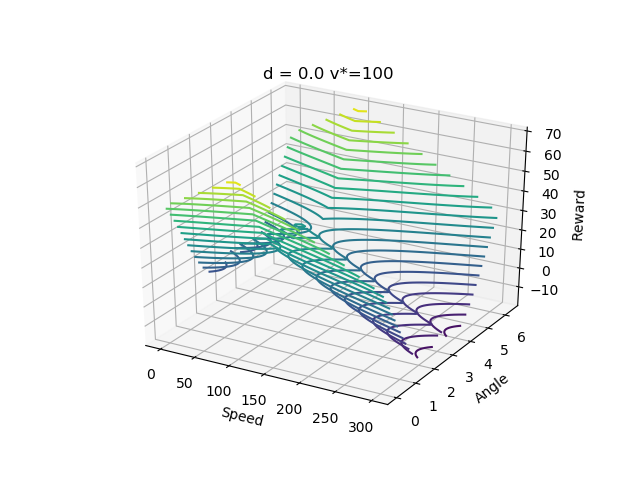
\includegraphics[width=0.7\textwidth]{reward_plot0}
  \caption{Plot of reward function for $trackPos = 1$ and $v^*=110$}
  \label{rewardshapingplot0}
\end{figure}
\begin{figure}[H]
  \centering
  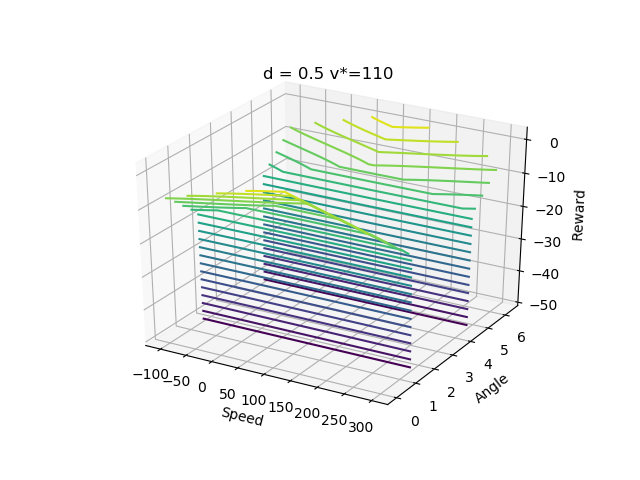
\includegraphics[width=0.7\textwidth]{reward_plot05}
  \caption{Plot of reward function for $trackPos = 1$ and $v^*=110$}
  \label{rewardshapingplot05}
\end{figure}
\begin{figure}[H]
  \centering
  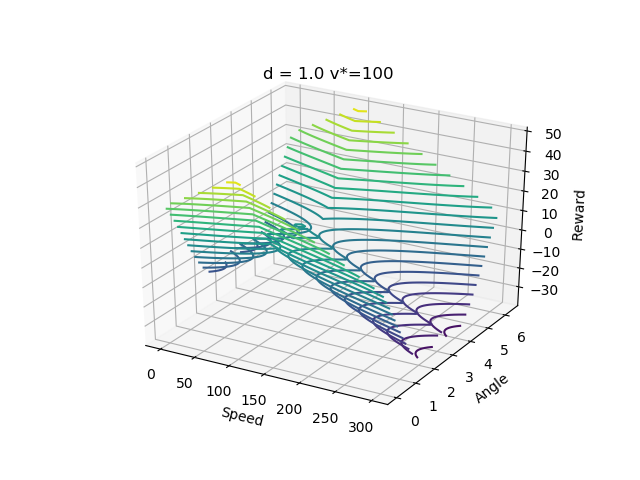
\includegraphics[width=0.7\textwidth]{reward_plot1}
  \caption{Plot of reward function for $trackPos = 1$ and $v^*=110$}
  \label{rewardshapingplot1}
\end{figure}
Figures \ref{rewardshapingplot0}, \ref{rewardshapingplot05} and \ref{rewardshapingplot1} show the plot of reward function for three values of $trackPos$ varying the speed and the angle. Since $trackPos$ is taken into account only with its absolute value, for negative values of $trackPos$ reward function is the same of the one for positive values. For $trackPos = 0$ the car is in the middle of the lane and the reward increases.



\chapter{Training and Evaluation}
The model has been trained for 500 episodes and it took about 2 hours. Car started moving randomly, which frequently led it out of track and achieving low reward. 

\begin{figure}[H]
  \centering
  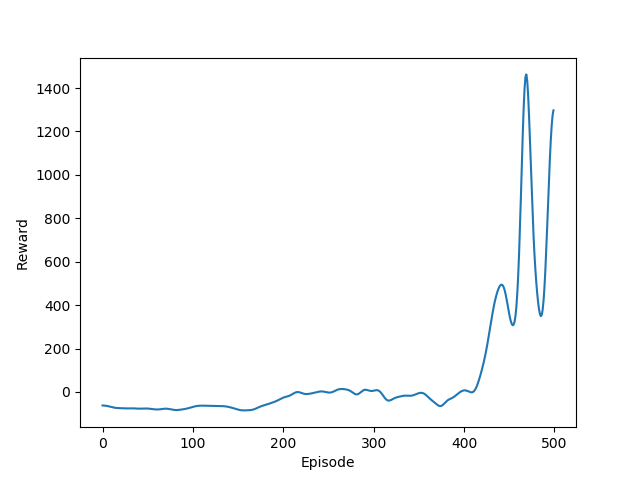
\includegraphics[width=.8\textwidth]{mean_reward}
  \caption{Episode Reward's Plot}
  \label{rewardplot}
\end{figure}

After about 400 episodes reward started increasing, since the car learned how to stay in the middle of the track: it understood how to use steering to minimize $trackPos$ and angle. The evolution of this two values is shown in Figures \ref{mean_trackpos} and \ref{mean_angle}. It is important to notice that both, and in particular the angle, stabilize around the $0$: this means that the car manages to keep the track.

\begin{figure}[H]
\centering
\caption{Car position sensors' plots}
\begin{subfigure}{.5\textwidth}
  \centering
  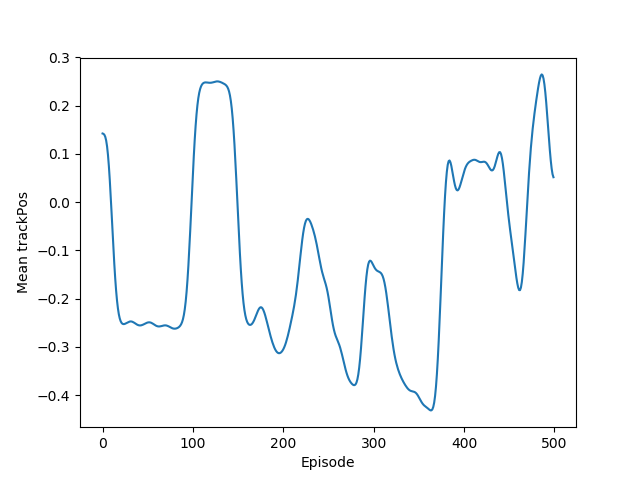
\includegraphics[width=.9\linewidth]{mean_trackpos}
  \caption{Mean trackPos plot}
  \label{mean_trackpos}
\end{subfigure}%
\begin{subfigure}{.5\textwidth}
  \centering
  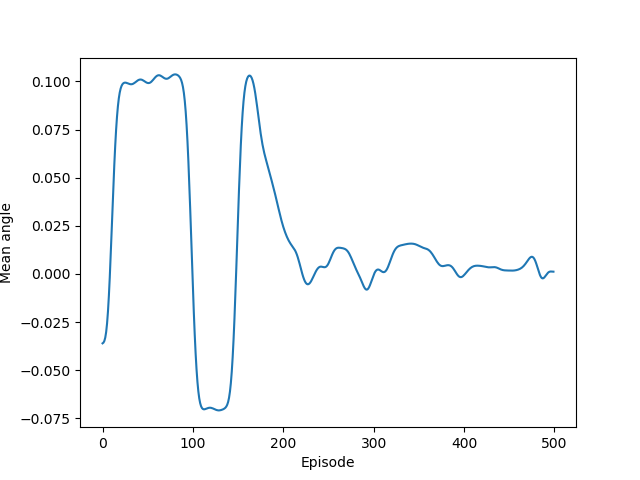
\includegraphics[width=.9\linewidth]{mean_angle}
  \caption{Mean angle plot}
  \label{mean_angle}
\end{subfigure}
\label{mean_plots}
\end{figure}
The maximum reward was reached when the agent learned to maintain a certain average speed, by balancing the throttle and the brake pedal. This last stage happened after the 450th episode: Figure \ref{mean_difference} shows the plot of the mean difference between car speed and specified one. It is important to notice that the error stabilizes around values smaller than $10$.
\begin{figure}[H]
  \centering
  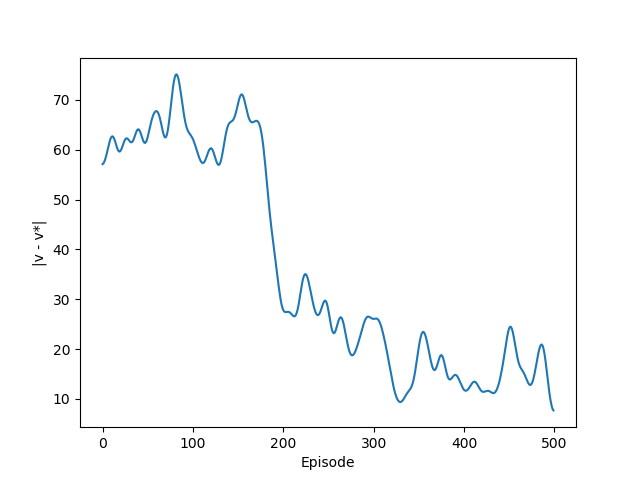
\includegraphics[width=.8\textwidth]{mean_difference}
  \caption{Mean average speed error}
  \label{mean_difference}
\end{figure}


% \begin{figure}[H]
% \centering
% \begin{subfigure}[H]{0.55\textwidth}
%   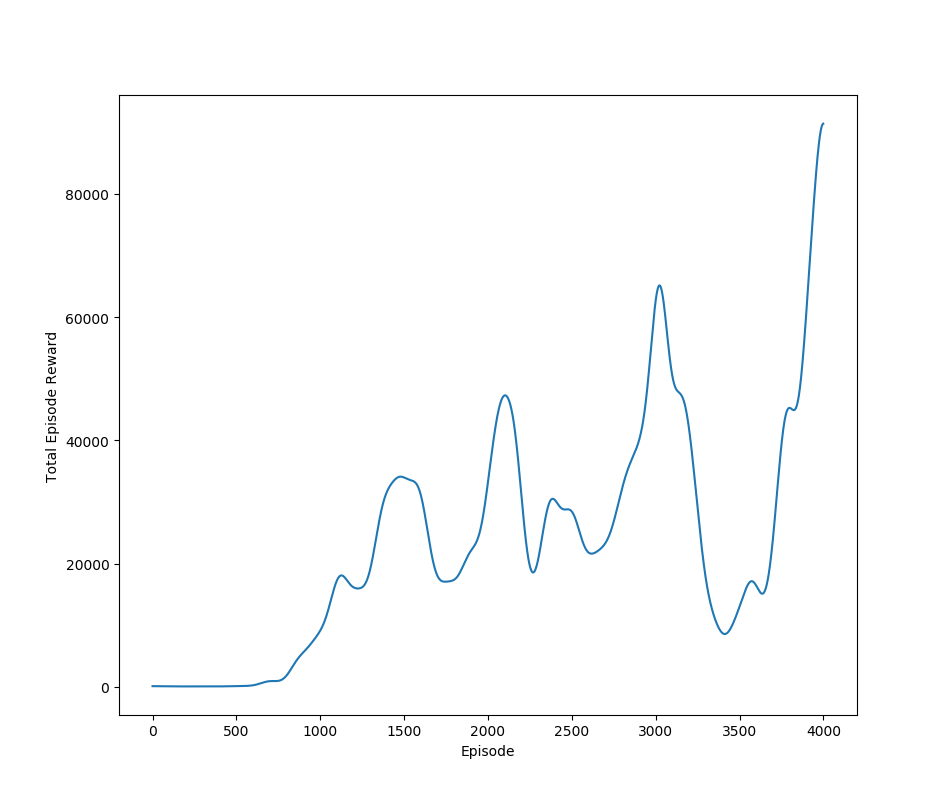
\includegraphics[width=1\linewidth]{reward}
%   \caption{Plot with linear y scale}
%   \label{rewardplot}
% \end{subfigure}\\
% \begin{subfigure}[H]{0.55\textwidth}
%   \centering
%   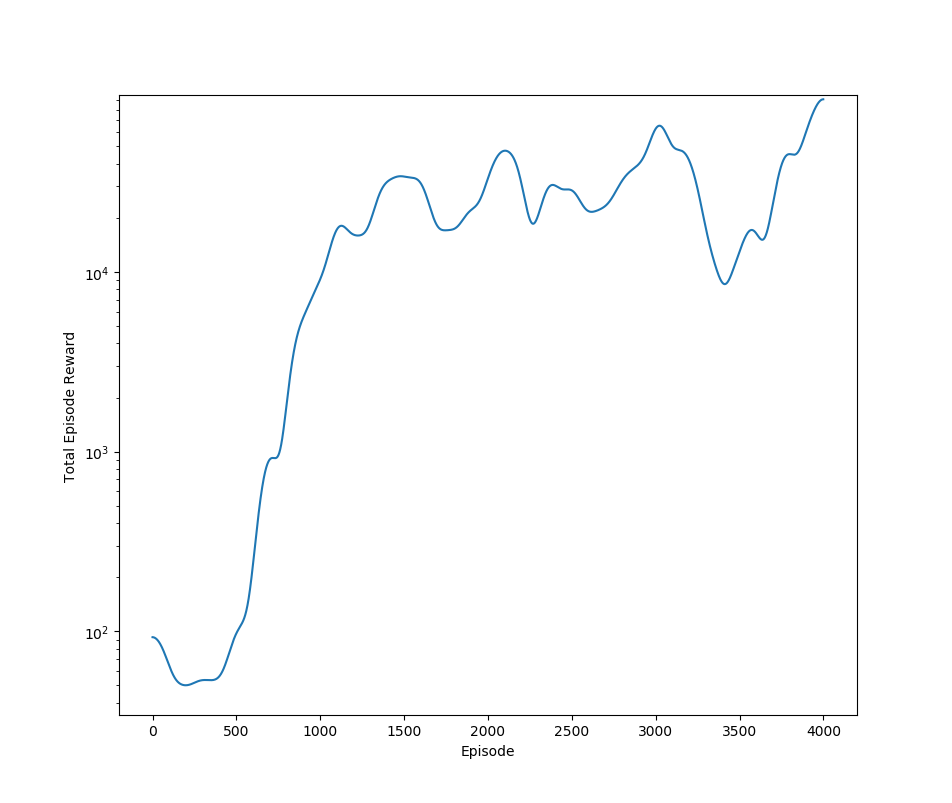
\includegraphics[width=1\linewidth]{rewardlog}
%   \caption{Plot with logarithmic y scale}
%   \label{rewardplotlog}
% \end{subfigure}
% \caption{Total Episode Reward Plots}
% \end{figure}

Due to OU process, the training total reward's plot appears quite noisy (Figure \ref{rewardplot}) but it shows clearly how the episode reward kept growing up during training.

The reward's plot noise could also be caused by the chosen reward shaping: during long episodes the agent accumulates high rewards, while during short ones (when it goes out of track early) negative reward has an high impact on total reward. This problem has been highlighted by Gal Dalal et al. in Safe Exploration in Continuous Action Spaces \cite{SAFEEXPLORATION} but it extremely depends on the environment.
\begin{figure}[H]
  \centering
  
\includegraphics[width=.2\textwidth]{g-track-1}
  \caption{CG Speedway number 1 Circuit}
  \label{g-track-1}
\end{figure}


The agent has been trained only on CG Speedway number 1 track (Figure \ref{g-track-1}), which is a medium level one: it has two bends of more than 90 degree angles and long straight parts. This allowed a good training for both maintaining the specified speed and avoiding to go out of track.
A screenshot of the agent driving on CG Speedway number 1 is shown in Figure \ref{screenshot}.
\begin{figure}[H]
  \centering
  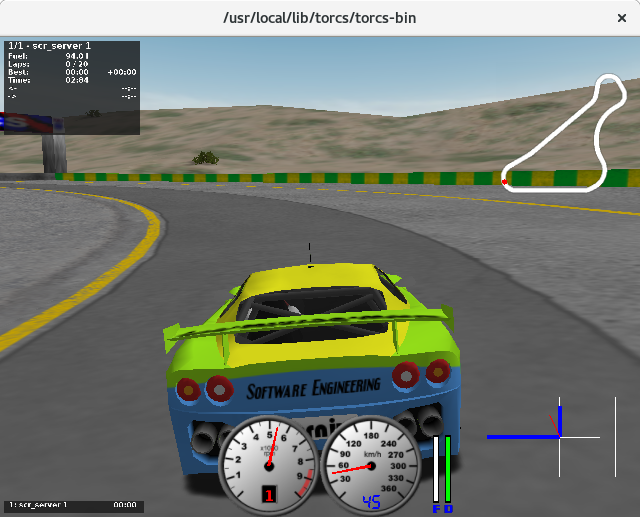
\includegraphics[width=.8\textwidth]{screenshot}
  \caption{CG Speedway number 1 screenshot}
  \label{screenshot}
\end{figure}
\chapter{Conclusions}
This project was meant to teach a car how to keep the track and maintain a certain speed. 

Reinforcement Learning and, in particular, Deep Deterministic Policy Gradient demonstrated to be powerful and fast algorithms to train agents in continuous state-action space.  

The agent trained on a single track resulted to be able to drive on different tracks and act very well maintaining  a specified speed. An improvement could be provided by adding the camera to the sensors, although it would be longer to train the model.

Car varied continuously throttle and steering, this led to driving jerky and sliding out of track. To fix this problem, it would be possible to use fixed variations of throttle and steering as actions instead their real values.

As explained by Gal Dalal et al. \cite{SAFEEXPLORATION} it would be possible to use a Safe Exploration Layer instead of Reward Shaping to teach the agent to stay in the track in order to reduce noise in training phase.

Taking into account the obtained results, it is possible to assert that the project purpose has been accomplished although some improvements could still be adopted in the future. 


\backmatter

\cleardoublepage
\phantomsection % Give this command only if hyperref is loaded
\addcontentsline{toc}{chapter}{\bibname}
\bibliography{tesi}{}
\bibliographystyle{unsrt}
% Here put the code for the bibliography. You can use BibTeX or
% the BibLaTeX package or the simple environment thebibliography.

\begin{acknowledgments}
I would not be where I am today if it wasn't for the support given from the people that have always been by my side during my life.

First of all, my gratification goes to my parents, without whom all this would have never happened.

I want to thank my sister Chiara, my family, my girlfriend Veronica and my friends, especially Dylan, who has been bearing me for eight years.

I'm very grateful to Prof. Capobianco, my Excellence Course Advisor, who made this project achievable.

Last but not least, thanks to Virginia who provided very helpful fixing for this thesis.
\end{acknowledgments}

\end{document}